\section{Estrutura Cristalina}

\subsection*{Material Amorfo X Cristalino}
O material CRISTALINO possui arranjo mais uniforme e as moléculas está direcionadas de forma a apresentarem um densidade molecular maior. 

O material AMORFO possui suas moléculas dispostas de forma mais aleatória e a densidade molecular dessa região é menor.


\subsection*{CRISTALINIDADE} Arranjo interno ordenado das partículas segundo um modelo tridimensional, característico do estado sólido. Em muitos corpos a cristalinidade é evidenciada por faces e simetria externa, indicando um arranjo ordenado dos átomos. Exames em raios X(1912) estudo de substâncias inorgânicas.

\subsection*{CRISTALOGRAFIA} Estudo dos corpos sólidos que possuem estrutura cristalina e das leis que governam seu crescimento, forma externa e interna. É instrumento fundamental na química, física, metalurgia e no estudos das cerâmicas, refratários, semicondutores, gemas sintéticas, etc.


\subsection*{CÉLULAS UNITÁRIAS} para a maioria dos cristais, as células unitárias podem ser representadas por geometrias específicas. Mais do que uma célula unitária pode ser escolhida para representar o cristal. Geralmente, escolhe-se a que apresenta o maior grau de simetria geométrica.



\subsection*{SISTEMAS CRISTALINOS} Qualquer empacotamento atômico deverá se encaixar em um dos sete principais tipos de cristais, que estão intimamente associados com o modo pelo qual o espaço pode ser dividido em volumes iguais, pela interseção de superfícies planas.
Existem diferentes estruturas cristalinas possíveis. É conveniente dividi-las em grupos de acordo com as configurações das células unitárias e/ou os arranjos atômicos. Para criar todos os tipos de redes são necessários sete tipos distintos de células cristalinas.


\section{Células unitárias e Sistemas cristalinos}

Parâmetros de rede cristalina:
\begin{itemize}
	\setlength{\parskip}{0pt}
	\setlength{\itemsep}{0pt plus 1pt}
	
	\item a,b,c - comprimentos dos lados do paralelepípedo
	\item $ \alpha$, $\beta$, $\gamma $ - ângulos entre os eixos
\end{itemize}




Com base nestes parâmetros de rede, tem-se que existem 7 diferentes combinações possíveis entre a,b,c e $\alpha, \beta, \gamma $ cada um representando um sistema cristalino.


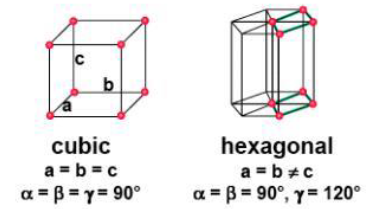
\includegraphics[scale=0.5,trim={0 0 0 0}]{figures/crist1}

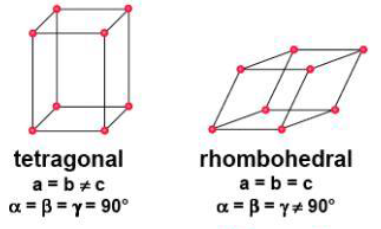
\includegraphics[scale=0.5,trim={0 0 0 0}]{figures/crist2}

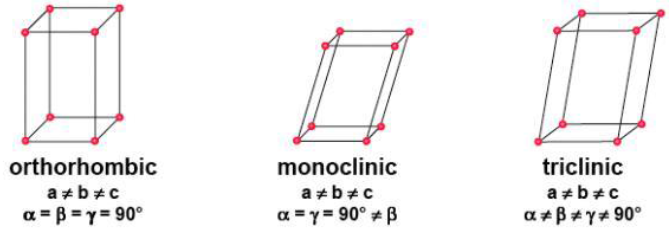
\includegraphics[scale=0.3,trim={0 0 0 0}]{figures/crist3}


O maior grau de simetria aparece no sistema cúbico e o menor grau é visto no sistema triclínico.

\subsection*{Variações na célula unitária básica}

As possíveis redes podem ser descritas por 14 células unitárias (A.J. Bravais).
Em algumas células unitárias existem alguns tipos básicos: simples, de corpo centrado e de faces centradas.
 
 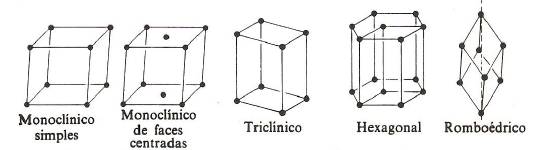
\includegraphics[scale=0.4,trim={0 0 0 0}]{figures/var1}
 
 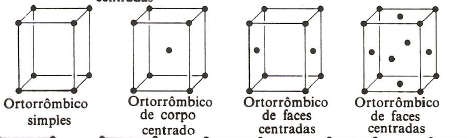
\includegraphics[scale=0.45,trim={0 0 0 0}]{figures/var2}
 
 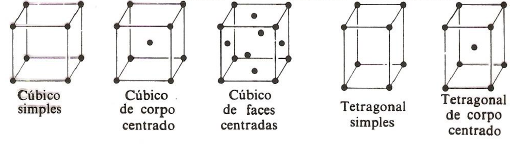
\includegraphics[scale=0.5,trim={0 0 0 0}]{figures/var3}



\subsection*{Características}

Numero de Coordenação: número de partículas que envolvem uma partícula central.

Fator de empacotamento: volume de átomos numa célula unitária / volume da célula unitária.

\subsection*{Valores para alguns sistemas cristalinos}

\begin{itemize}
	\setlength{\parskip}{0pt}
	\setlength{\itemsep}{0pt plus 1pt}
	
	\item NC: Número de Coordenação
	\item FE: Fator de empacotamento
\end{itemize}


Cubo simples - CS




\begin{itemize}
	\item NC: 6;
	\item FE: $\frac{4}{3} \cdot \frac{\pi \cdot r^{3}}{a^{3}} = 0,52$;
	\item Rel: $a = 2R$;	
\end{itemize}


Cúbico de Corpo Centrado - CCC

\begin{itemize}
	\item NC: 8
	\item FE: $2 \cdot \frac{4}{3} \cdot \frac{\pi \cdot r^{3}}{a^{3}} = 0,68$
	\item Rel: $a = \frac{4R}{\sqrt{3}}$
\end{itemize}


Cúbico de Faces Centradas - CFC

\begin{itemize}
	\setlength{\parskip}{0pt}
	\setlength{\itemsep}{0pt plus 1pt}
	
	\item NC: 12
	\item FE: $4 \cdot \frac{4}{3} \cdot \frac{\pi \cdot r^{3}}{a^{3}}$ 0,74
	\item Rel: a = $\frac{4 \cdot R}{\sqrt{2}}$
\end{itemize}

Hexagonal

\begin{itemize}
	
	\setlength{\parskip}{0pt}
	\setlength{\itemsep}{0pt plus 1pt}
	
	\item NC: 12
	\item FE: 0,73 (=CFC)
	\item Rel: a = 2R
\end{itemize}


 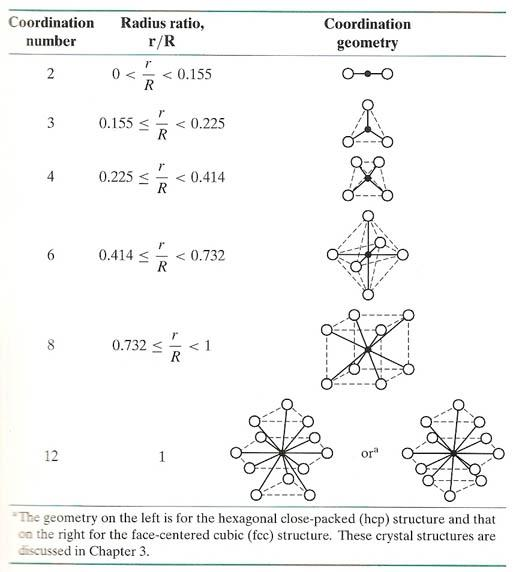
\includegraphics[scale=0.3,trim={0 0 0 0}]{figures/RELraio}
 
 
 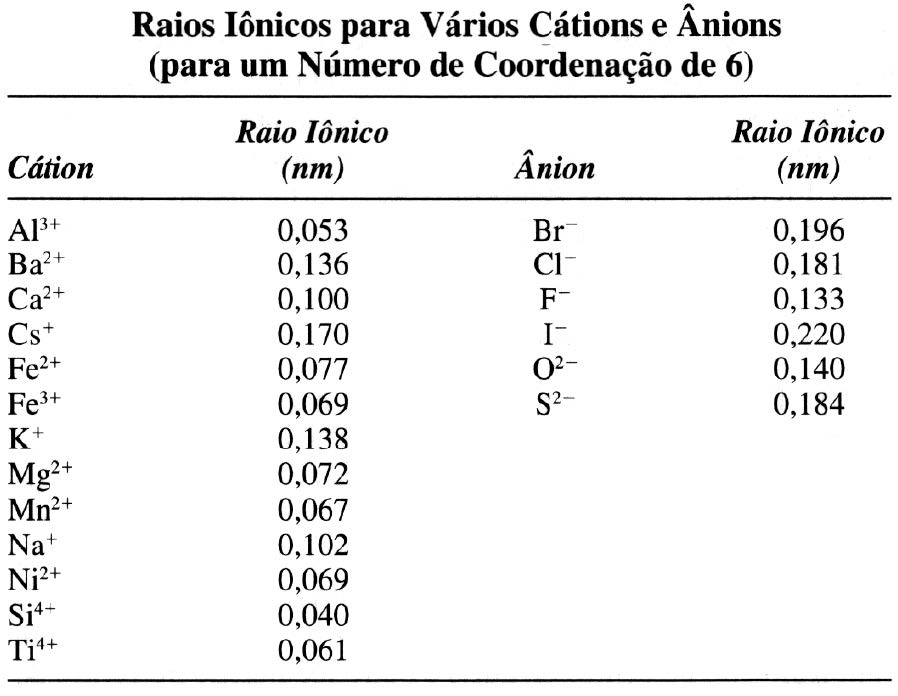
\includegraphics[scale=0.25,trim={0 0 0 0}]{figures/raio}
 

 \section{Estrutura dos materiais Cerâmicos}
 
O posicionamento das partículas nos materiais cerâmicos depende da relação entre os raios(cátion/ânion) e das cargas envolvidas. Nos vazios (sítios ou interstícios) da rede cristalina se posicionam partículas diferentes das que existem na rede cristalina principal. Em redes compactas há espaços intersticiais, onde as partículas ficam equidistantes do centro do espaço vazio.
 

\textbf{Posições octaédricas na rede cfc:}

 \begin{itemize}
 	
 	\setlength{\parskip}{0pt}
 	\setlength{\itemsep}{0pt plus 1pt}
 	
 	\item NC: 6
 	\item Local:arestas (3 sítios) + centro da célula unitária
 	\item Total: 4 partículas (1 por partículas da célula unitária)
 \end{itemize}

 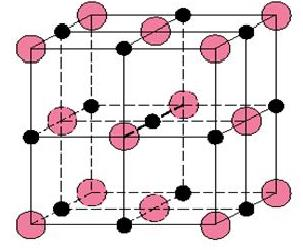
\includegraphics[scale=0.5,trim={0 0 0 0}]{figures/occfc}
 
 
\textbf{ Posições tetraédricas na rede cfc:}

  \begin{itemize}
 	
 	\setlength{\parskip}{0pt}
 	\setlength{\itemsep}{0pt plus 1pt}
 	
 	\item NC: 4
 	\item Local:posições do tipo ($\frac{1}{4}$, $\frac{1}{4}$, $\frac{1}{4}$)
 	\item Total: 8 partículas (2 por partículas	da célula unitária)
 \end{itemize}

 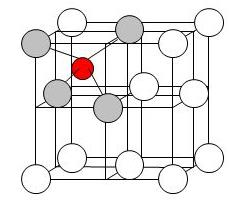
\includegraphics[scale=0.5,trim={0 0 0 0}]{figures/tetcfc}
 
\section{Estrutura dos Materiais Cerâmicos}
FEI=fator de empacotamento iônico
As estruturas são bastante complexas, podendo-se representar alguns tipos mais comuns:


\begin{itemize}
	\item Cerâmicostipo MaM’bXc
	\item $MX$
	\item $MX_{2}$
	\item $M_{2}X_{3}$
	\item $MM'X_{3}$
	\item $M'M_{2}''X_{4}$
\end{itemize}

M –elemento metálico

X–elemento não-metálico



Estrutura tipo MX -NaCl

Ex 1: NaCl (cfc)
NC = 6
A estrutura pode ser vista como duas estruturas CFC, uma de íons sódio e uma de íons cloro.
2 íons associados(1 Na+e 1 Cl-)
4 íons de cada (CFC –4 átomos por célula unitária)
São 8 íons por célula unitária.
Outros compostos com esta estrutura: CaO, NiO, FeO, MgO.

 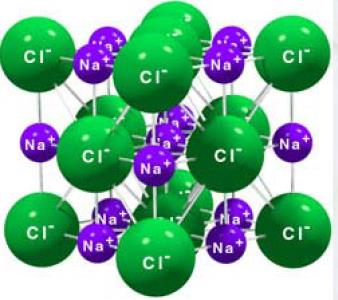
\includegraphics[scale=0.5,trim={0 0 0 0}]{figures/NaCl}


Estrutura tipo MX -CsCl
Ex2: CsCl(ccc)

Estrutura cúbica (NC = 8)

 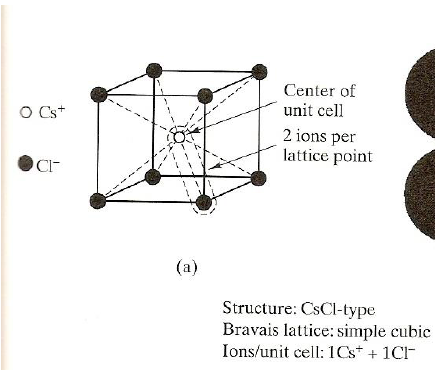
\includegraphics[scale=0.2,trim={0 0 0 0}]{figures/CsCl}
 
 

Estrutura tipo MX -ZnS
Ex3: ZnS(cfc)
cfc:8 íons por célula unitária (4 Zn2+e 4 S2-)
4 S2-em posição cfce Zn2+em 4 sítios tetraédricos
(1/2 dos sítios tetraédricos ocupados)

 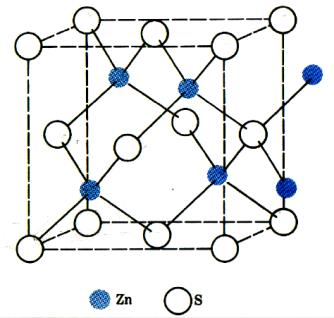
\includegraphics[scale=0.3,trim={0 0 0 0}]{figures/ZnS}


 Estrutura tipo MX2 –CaF2
 Ex: CaF2(cfc) -FLUORITA
 
3 íons associados ($1Ca^{+2} e 2F^{-}$)
4 íons Ca+2 (estrutura cfc) e 8 íons F-(12 íons por célula unitária)
Volume não preenchido próximo ao centro da célula unitária.

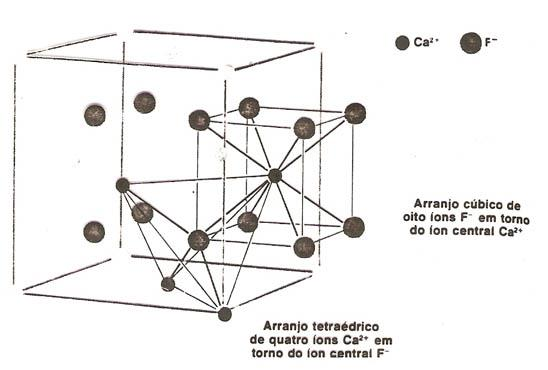
\includegraphics[scale=0.3,trim={0 0 0 0}]{figures/CaF2}

Estrutura tipo M2X3

Ex: Al2O3–alumina ou corundum
30 íons por célula unitária (12Al+3e18O2-)
2/3 dos interstícios ocupados por íons alumínio.
Outros compostos com esta estrutura:-Fe2O3,Cr2O3.
  
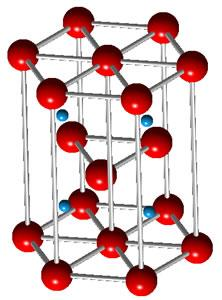
\includegraphics[scale=0.5,trim={0 0 0 0}]{figures/Al2O3}

Estrutura tipo MM'X3

 MeM'– elementos metálicos
 X –elemento não-metálico
 Ex: CaTiO3(combinação de estruturas cs, cc, cfc)–importante família de materiais cerâmicos usados na indústria eletrônica (propriedades piezoelétricas).
 Ca+2nos vértices, Ti+4como corpo centrado e O2-na faces.
 Este tipo de rede é um exemplo da estrutura CS formada pelos íons cálcio.
 Existem 5 íons por célula unitária (1Ca+2,1Ti4+e3O2)
 Outro composto com esta estrutura: BaTiO3.
 
  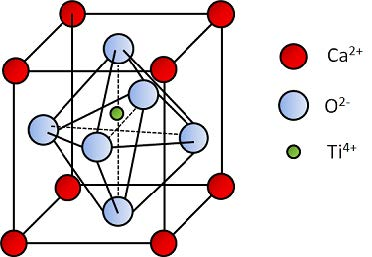
\includegraphics[scale=0.5,trim={0 0 0 0}]{figures/CaTiO}
  
  
Estrutura tipo MM2'X4

M(valência+2)eM'(valência+3)–elementos metálicos
X –elemento não-metálico
Ex: MgAl2O4(cfc)-importante família de materiais cerâmicos magnéticos (espinélios).
56 íons por célula unitária (8Mg+2,16Al3+e32O2-),
Outros compostos com esta estrutura: NiAl2O4,MgAl2O4,ZnFe2O4.

 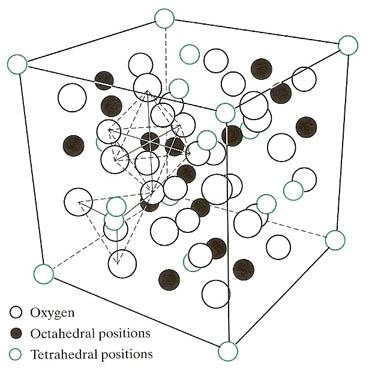
\includegraphics[scale=0.3,trim={0 0 0 0}]{figures/MgAlO}

\section{Estruturasdos Silicatos}
Formam a classe máxima entre os minerais.

\begin{itemize}
	\item A estrutura é complexa, não podendo ser definida como um tipo simples de estrutura, variando em função da temperatura e pressão.
	\item A característica geral dos silicatos é a mesma (tetraedros unidos) diferenciando em relação ao compartilhamento dos oxigênios.
\end{itemize}

Várias estruturas de silicatos surgem das diferentes maneiras segundo as quais unidades de (SiO4)-4 se unem formando arranjos unidimensionais, bidimensionais e tridimensionais.

Para Desenhar e anotar


Para os vários minerais à base de silicatos, 1, 2 ou 3 átomos de oxigênio nos vértices dos tetraedros são compartilhados por outros tetraedros para formar estruturas complexas.

Podem conter vários elementos em combinação com o silício e o oxigênio (ex: Na, K, Ca, Mg, Al e Fe).

 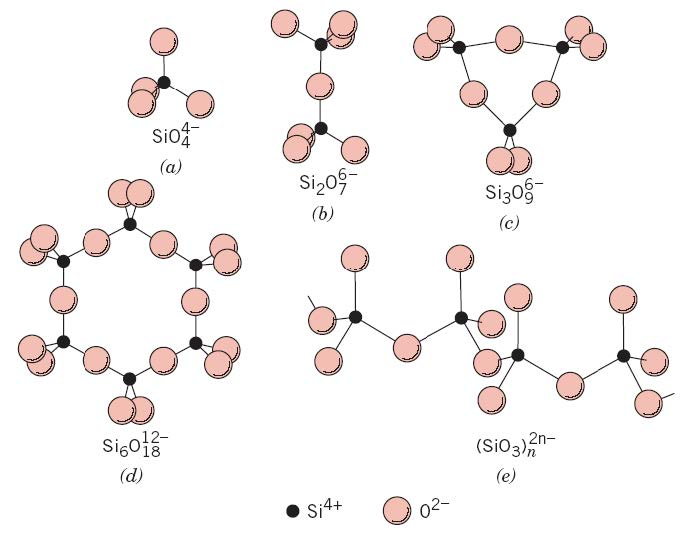
\includegraphics[scale=0.3,trim={0 0 0 0}]{figures/estsil}
  
 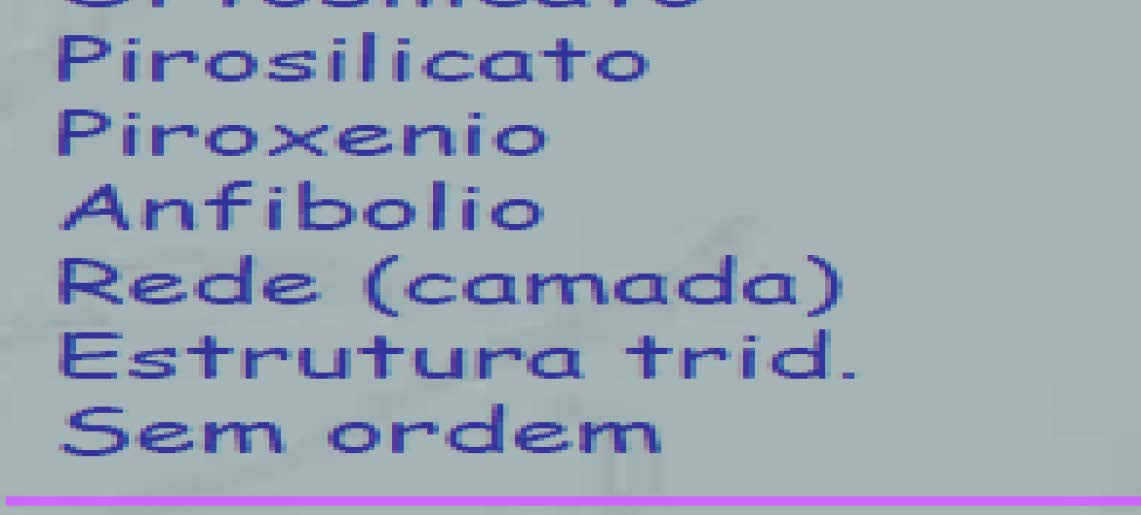
\includegraphics[scale=0.25,trim={0 0 0 0}]{figures/sil1}

\begin{itemize}
	\item tetraedros simples - ex: Mg2SiO4
	\item tetraedros duplos - ex: Zn4(Si2O7)(OH)2.H2O)
	\item anéis (unidade estrutural (SiO3)–2 )
	\item camadas - ex: talco: Mg3(Si2O5)2(H2O))
	\item redes (feldspatos, zeólitas, quartzo: SiO2) )
\end{itemize}

\textbf{Ex 1:SiO2(cfc) -CRISTOBALITA}
6 íons associados (2 Si+4e 4 O-2): Si2O4
24 íons por célula unitária(8 Si+4e 16 O-2)
Apesar da grande célula unitária necessária para descrever a estrutura, é uma das formas mais simples do SiO2.


\textbf{Ex2: Grupo dos feldspatos}

X Al(1-2)Si(2-3) O8


onde: Quando X tem carga +1, há 1Al e 3Si X = Na+, K+ou Ca2+ Quando X tem carga +2, há 2Al e 2Si. Quanto maior a quantidade de Ca, maior a quantidade de Al no feldspato. Os Si e os Al ocupam os centros de tetraedros interconectados. Os cátions X se situam nos vazios da estrutura.



\textbf{Ex3: Alumino-silicatos}
Alumínio pode entrar em Coordenação tetraédrica(em substituição ao Si) ou em Coordenação octaédrica, unindo tetraedros.
Mg2+, Fe2+, Fe3+, Mn2+, Al3+e o Ti4+tendem a ocorrer nas estruturas dos silicatos em coordenação octaédrica (em relação ao O2-).
Ca2+ (0,99 Å) e Na+(0,97 Å) (cátions maiores e de carga mais fraca) entram em coordenação cúbica (NC = 8).
Se um cátion trivalente substitui um tetravalente, ex: Fe3+na posição do Ti4+, outra substituição tem de ser feita no cristal de forma a perder uma carga positiva ou ganhar uma negativa eletroneutralidade.


\textbf{Ex4: Sílica vítrea}
SiO2 sem arranjo cristalino regular
